% THIS DOCUMENT IS FOLLOWS THE VOLERE TEMPLATE BY Suzanne Robertson and James Robertson
% ONLY THE SECTION HEADINGS ARE PROVIDED
%
% Initial draft from https://github.com/Dieblich/volere
%
% Risks are removed because they are covered by the Hazard Analysis
\documentclass[12pt]{article}

\usepackage{booktabs}
\usepackage{tabularx}
\usepackage{longtable}
\usepackage{graphicx}
\usepackage{hyperref}
\usepackage{float}
\graphicspath{ {./res/} }
\hypersetup{
    bookmarks=true,         % show bookmarks bar?
      colorlinks=true,      % false: boxed links; true: colored links
    linkcolor=red,          % color of internal links (change box color with linkbordercolor)
    citecolor=green,        % color of links to bibliography
    filecolor=magenta,      % color of file links
    urlcolor=cyan           % color of external links
}

\newcommand{\lips}{\textit{Insert your content here.}}

%% Comments

\usepackage{color}

\newif\ifcomments\commentstrue %displays comments
%\newif\ifcomments\commentsfalse %so that comments do not display

\ifcomments
\newcommand{\authornote}[3]{\textcolor{#1}{[#3 ---#2]}}
\newcommand{\todo}[1]{\textcolor{red}{[TODO: #1]}}
\else
\newcommand{\authornote}[3]{}
\newcommand{\todo}[1]{}
\fi

\newcommand{\wss}[1]{\authornote{blue}{SS}{#1}} 
\newcommand{\plt}[1]{\authornote{magenta}{TPLT}{#1}} %For explanation of the template
\newcommand{\an}[1]{\authornote{cyan}{Author}{#1}}

%% Common Parts

\newcommand{\progname}{ProgName} % PUT YOUR PROGRAM NAME HERE
\newcommand{\authname}{Team \#, Team Name
\\ Student 1 name
\\ Student 2 name
\\ Student 3 name
\\ Student 4 name} % AUTHOR NAMES                  

\usepackage{hyperref}
    \hypersetup{colorlinks=true, linkcolor=blue, citecolor=blue, filecolor=blue,
                urlcolor=blue, unicode=false}
    \urlstyle{same}
                                


\begin{document}

\title{Software Requirements Specification for \progname: subtitle describing software} 
\author{\authname}
\date{\today}
	
\maketitle

~\newpage

\pagenumbering{roman}

\tableofcontents

~\newpage

\section*{Revision History}

\begin{tabularx}{\textwidth}{p{3cm}p{2cm}X}
\toprule {\textbf{Date}} & {\textbf{Version}} & {\textbf{Notes}}\\
\midrule
Date 1 & 1.0 & Notes\\
Date 2 & 1.1 & Notes\\
\bottomrule
\end{tabularx}

~\\

~\newpage
\section{Purpose of the Project}
\subsection{User Business}
\lips
\subsection{Goals of the Project}
\lips
\section{Stakeholders}
\subsection{Client}
\lips
\subsection{Customer}
\lips
\subsection{Other Stakeholders}
\lips
\subsection{Hands-On Users of the Project}
\lips
\subsection{Personas}
\lips
\subsection{Priorities Assigned to Users}
\lips
\subsection{User Participation}
\lips
\subsection{Maintenance Users and Service Technicians}
\lips

\section{Mandated Constraints}
\subsection{Solution Constraints}
\lips
\subsection{Implementation Environment of the Current System}
\lips
\subsection{Partner or Collaborative Applications}
\lips
\subsection{Off-the-Shelf Software}
\lips
\subsection{Anticipated Workplace Environment}
\lips
\subsection{Schedule Constraints}
\lips
\subsection{Budget Constraints}
\lips
\subsection{Enterprise Constraints}
\lips

\section{Naming Conventions and Terminology}
\subsection{Glossary of All Terms, Including Acronyms, Used by Stakeholders
involved in the Project}
\lips

\section{Relevant Facts And Assumptions}
\subsection{Relevant Facts}
\lips
\subsection{Business Rules}
\lips
\subsection{Assumptions}
\lips

\section{The Scope of the Work}
\subsection{The Current Situation}
\begin{figure}[H]
    \centering
    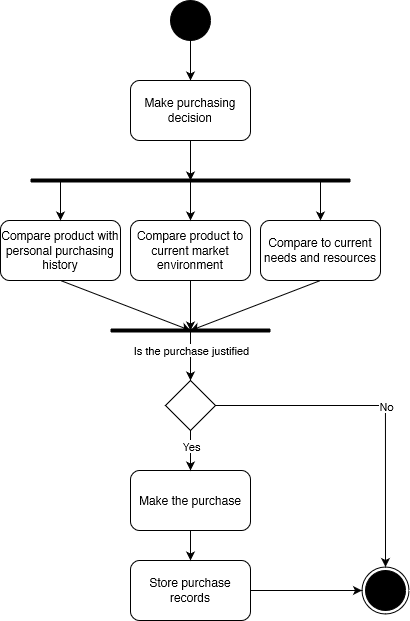
\includegraphics[width=0.6\textwidth]{currentsituation}
    \caption{Current Situation Activity Diagram}
    \label{fig:currentsituation}
\end{figure}
\subsection{The Context of the Work}
\begin{figure}[H]
    \centering
    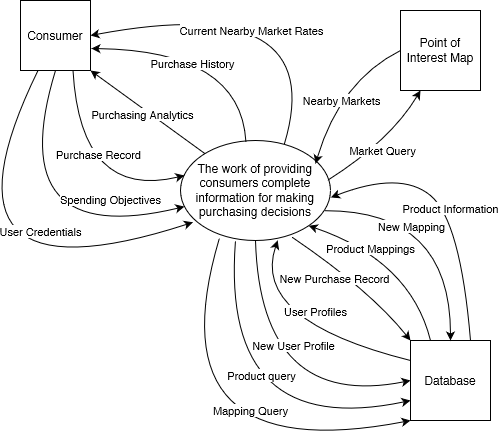
\includegraphics[width=0.9\textwidth]{workcontext}
    \caption{Work Context Model}
    \label{fig:workcontext}
\end{figure}
\subsection{Work Partitioning}
    \begin{longtable}{| >{\raggedright\arraybackslash}p{.30\textwidth} | >{\raggedright\arraybackslash}p{.30\textwidth} | >{\raggedright\arraybackslash}p{.30\textwidth} |}
        \hline
        \textbf{Event Name} & \textbf{Input/output} & \textbf{Summary of BUC} \\
        \hline
        User inputs user profile credentials & User Credentials (in) & Initialize user profile from received credentials \\
        \hline
        Consumer inputs spending objectives & Spending objectives (in) & Records the objectives and the owner \\
        \hline
        Consumer inputs purchase record & Purchase record (in) & Records the purchase and the owner of the purchase \\
        \hline
        User requests purchasing analytics & Purchasing analytics (out) & Report compiled and computed information from available data for the user profile \\
        \hline
        User requests personal purchase history & Purchase history (out) & Report compiled user purchasing history\\
        \hline
        User requests information on a product & Current nearby market rates (out) & Report market rates for a product that is accessible to the user \\
        \hline
        Compiling market information relevant to a user & Nearby markets (in) & Record information for accessible markets based on criteria \\
        \hline
        Request information on markets & Market query (out) & Send request for market information under a set of specified parameters \\
        \hline
        Database transmits product information & Product information (out) & Record information on product \\
        \hline
        New mapping received & Mapping Data (out) & Send new good/service mapping to database \\
        \hline
        Database transmits requested mapping data & Product mappings (in) & Record the product mappings \\
        \hline
        Send purchase record to database & New purchase record (out) &  Send purchase record to database \\
        \hline
        Database transmits requested user profile data & User profiles (in) &  Record the user profile data \\
        \hline
        Send user profile data & New user profile (out) &  Send a user profile to database \\
        \hline
        Send product query to database & Product query (out) & Request relevant data based on product query from database \\
        \hline
        Send mapping query to database  & Mapping query (out) &  Request relevant data based on mapping query from database \\
        \hline 
        \caption{Business Event List}
        \label{tab:businesseventlist}
    \end{longtable}
\subsection{Specifying a Business Use Case (BUC)}
\textbf{Title:} Create a new profile\\
\textbf{Trigger:} User creates a new profile\\
\textbf{Pre-condition:} User has application running\\
\textbf{Outcome: } 
\begin{enumerate}
    \item User creates an profile identified by a username and a password
    \item System creates new profile entry in database
\end{enumerate}
\textbf{Title:} Log in to user profile\\
\textbf{Trigger:} User submits profile credentials \\
\textbf{Pre-condition:} Profile exists in database \\
\textbf{Outcome: } 
\begin{enumerate}
    \item System checks if profile credentials exists
    \item If exists, system allows loads user profile
    \item If not exists, systems shows error message
\end{enumerate}
\textbf{Title:} Record user objectives \\
\textbf{Trigger:} User submits personal objectives \\
\textbf{Pre-condition:} User is logged into profile \\
\textbf{Outcome: } 
\begin{enumerate}
    \item System stores user budgeting objectives of budget with associated product or product groups
\end{enumerate}
\textbf{Title:} Input purchase records \\
\textbf{Trigger:} User submits image or manual entry of purchase record \\
\textbf{Pre-condition:} User is logged into profile \\
\textbf{Outcome: } 
\begin{enumerate}
    \item System reads and translates records to Strings
    \item System maps input records to database objects
    \item If mapping does not exist, make guesses and prompt user for feedback
    \item Save records to database
\end{enumerate}
\textbf{Title:} Create new mapping feedback \\
\textbf{Trigger:} Product mapping is not found in database \\
\textbf{Pre-condition:} Product record has been submitted \\
\textbf{Outcome: } 
\begin{enumerate}
    \item Create mapping guesses using language model
    \item Prompt user with guesses for feedback
    \item User inputs feedback
    \item Process and screen user feedback
    \item If mapping is eligible, create new mapping entry in database
\end{enumerate}
\textbf{Title:} Create user profile analytics \\
\textbf{Trigger:} User requests purchasing analytics \\
\textbf{Pre-condition:} User is logged into profile \\
\textbf{Outcome: } 
\begin{enumerate}
    \item Retrieve user data from database
    \item Transform user profile data into graphics
    \item Display graphics in application
\end{enumerate}
\textbf{Title:} Retrieve profile purchase history \\
\textbf{Trigger:} User requests purchase history\\
\textbf{Pre-condition:} User is logged into profile\\
\textbf{Outcome: } 
\begin{enumerate}
    \item Retrieve user purchase history from database
    \item Transform user purchase history into graphics
    \item Display graphics in application
\end{enumerate}
\textbf{Title:} Retrieve product information \\
\textbf{Trigger:} User requests product information\\
\textbf{Pre-condition:} User is logged into profile and has current location information set \\
\textbf{Outcome: } 
\begin{enumerate}
    \item Retrieve user purchase history from database relevant to the product
    \item Retrieve markets accessible to the user from map service
    \item Retrieve product information belonging to the accessible markets from database
    \item Transform data into graphics
    \item Display graphics in application
\end{enumerate}
\textbf{Title:} Set location information \\
\textbf{Trigger:} User sets location information \\
\textbf{Pre-condition:} User is logged into profile and location information is available \\
\textbf{Outcome: } 
\begin{enumerate}
    \item User sets initial location
    \item User sets accessibility radius
    \item Information is stored locally on device
\end{enumerate}

\section{Business Data Model and Data Dictionary}
\subsection{Business Data Model}
\lips
\subsection{Data Dictionary}
\lips

\section{The Scope of the Product}
\subsection{Product Boundary}
\lips
\subsection{Product Use Case Table}
\lips
\subsection{Individual Product Use Cases (PUC's)}
\lips

\section{Functional Requirements}
\subsection{Functional Requirements}
\lips

\section{Look and Feel Requirements}
\subsection{Appearance Requirements}
\lips
\subsection{Style Requirements}
\lips

\section{Usability and Humanity Requirements}
\subsection{Ease of Use Requirements}
\lips
\subsection{Personalization and Internationalization Requirements}
\lips
\subsection{Learning Requirements}
\lips
\subsection{Understandability and Politeness Requirements}
\lips
\subsection{Accessibility Requirements}
\lips

\section{Performance Requirements}
\subsection{Speed and Latency Requirements}
\lips
\subsection{Safety-Critical Requirements}
\lips
\subsection{Precision or Accuracy Requirements}
\lips
\subsection{Robustness or Fault-Tolerance Requirements}
\lips
\subsection{Capacity Requirements}
\lips
\subsection{Scalability or Extensibility Requirements}
\lips
\subsection{Longevity Requirements}
\lips

\section{Operational and Environmental Requirements}
\subsection{Expected Physical Environment}
\lips
\subsection{Wider Environment Requirements}
\lips
\subsection{Requirements for Interfacing with Adjacent Systems}
\lips
\subsection{Productization Requirements}
\lips
\subsection{Release Requirements}
\lips

\section{Maintainability and Support Requirements}
\subsection{Maintenance Requirements}
\lips
\subsection{Supportability Requirements}
\lips
\subsection{Adaptability Requirements}
\lips

\section{Security Requirements}
\subsection{Access Requirements}
\lips
\subsection{Integrity Requirements}
\lips
\subsection{Privacy Requirements}
\lips
\subsection{Audit Requirements}
\lips
\subsection{Immunity Requirements}
\lips

\section{Cultural Requirements}
\subsection{Cultural Requirements}
\lips

\section{Compliance Requirements}
\subsection{Legal Requirements}
\lips
\subsection{Standards Compliance Requirements}
\lips

\section{Open Issues}
\lips

\section{Off-the-Shelf Solutions}
\subsection{Ready-Made Products}
\lips
\subsection{Reusable Components}
\lips
\subsection{Products That Can Be Copied}
\lips

\section{New Problems}
\subsection{Effects on the Current Environment}
\lips
\subsection{Effects on the Installed Systems}
\lips
\subsection{Potential User Problems}
\lips
\subsection{Limitations in the Anticipated Implementation Environment That May
Inhibit the New Product}
\lips
\subsection{Follow-Up Problems}
\lips

\section{Tasks}
\subsection{Project Planning}
\lips
\subsection{Planning of the Development Phases}
\lips

\section{Migration to the New Product}
\subsection{Requirements for Migration to the New Product}
\lips
\subsection{Data That Has to be Modified or Translated for the New System}
\lips

\section{Costs}
\lips
\section{User Documentation and Training}
\subsection{User Documentation Requirements}
\lips
\subsection{Training Requirements}
\lips

\section{Waiting Room}
\lips

\section{Ideas for Solution}
\lips

\newpage{}
\section*{Appendix --- Reflection}

The information in this section will be used to evaluate the team members on the
graduate attribute of Lifelong Learning.  Please answer the following questions:

\begin{enumerate}
  \item What knowledge and skills will the team collectively need to acquire to
  successfully complete this capstone project?  Examples of possible knowledge
  to acquire include domain specific knowledge from the domain of your
  application, or software engineering knowledge, mechatronics knowledge or
  computer science knowledge.  Skills may be related to technology, or writing,
  or presentation, or team management, etc.  You should look to identify at
  least one item for each team member.
  \item For each of the knowledge areas and skills identified in the previous
  question, what are at least two approaches to acquiring the knowledge or
  mastering the skill?  Of the identified approaches, which will each team
  member pursue, and why did they make this choice?
\end{enumerate}

\end{document}